\chapter{Radial Basis Function (RBF) Kernel SVM}
\label{chap:rbf_svm}

In this chapter, we evaluate the Radial Basis Function (RBF) Kernel. Unlike the polynomial kernel which maps data to a finite-degree polynomial space, the RBF kernel maps the data into an infinite-dimensional feature space, allowing the SVM to compute highly complex, localized, and non-linear decision boundaries. 

The RBF Kernel is mathematically defined as:
\begin{equation}
    k(x_1, x_2) = e^{-\gamma ||x_1 - x_2||^2} + \xi
\end{equation}
Because the kernel relies on an additional hyperparameter $\gamma$ (which dictates the radius of influence of the support vectors), we perform a 2D Grid Search, evaluating four values of $\gamma \in \{10^{-4}, 10^{-3}, 10^{-2}, 10^{-1}\}$ across a logarithmic sweep of $C \in [10^{-3}, 10^2]$. We use $K=1.0$ (where $\xi = K^2 = 1.0$) to account for the bias.

\section{Experimental Results (Grid Search)}

\subsection*{What do you obtain when applying the RBF Kernel across different $\gamma$ values?}

The evaluation on the target application ($\pi_T = 0.1$) yields the comprehensive trends plotted in Figure \ref{fig:rbf_svm}.

\begin{figure}[H]
    \centering
    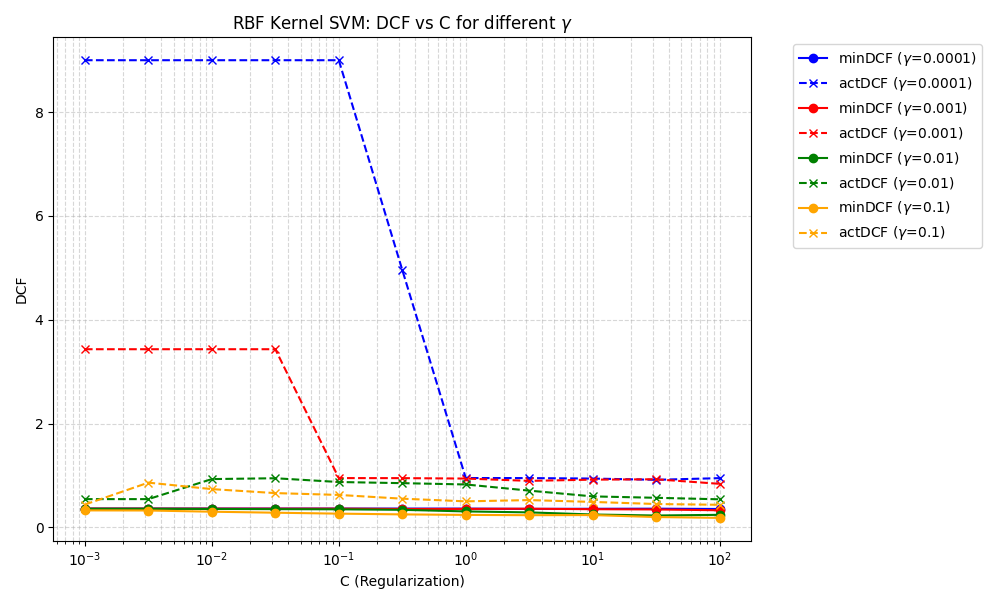
\includegraphics[width=0.85\textwidth]{RBF_Kernel_SVM_DCF_vs_C.png}
    \caption{Actual DCF and Minimum DCF as a function of $C$ across multiple $\gamma$ values for the RBF Kernel SVM ($K=1.0, \pi_T = 0.1$).}
    \label{fig:rbf_svm}
\end{figure}

The empirical logs reveal a clear hierarchy of performance dictated by $\gamma$:
\begin{itemize}
    \item \textbf{Low $\gamma$ ($10^{-4}$ and $10^{-3}$):} At these values, the model struggles to improve upon the linear baseline. For $\gamma = 10^{-4}$, the minimum DCF stalls around $0.3560$ even at maximum regularization ($C=10^2$). For $\gamma = 10^{-3}$, the model performs slightly better, reaching a minDCF of $0.3312$.
    \item \textbf{Moderate $\gamma$ ($10^{-2}$):} The discriminatory power drastically improves, mimicking the success of the quadratic kernel. The minDCF reaches $0.2303$ at $C=32.0$.
    \item \textbf{High $\gamma$ ($10^{-1}$):} At the highest evaluated $\gamma$, the model achieves an exceptionally low minDCF of \textbf{0.1845} at $C=10^2$, representing the strongest ranking capability observed so far. However, the Actual DCF at this operating point sits at $0.4367$, indicating a significant loss of calibration.
\end{itemize}

\section{Analysis and Considerations}

\subsection*{How does $\gamma$ affect the complexity of the decision boundary?}

The parameter $\gamma$ fundamentally controls the smoothness and locality of the separating boundary:
\begin{itemize}
    \item A \textbf{low $\gamma$} means the exponential function decays very slowly. Consequently, the "radius of influence" of each support vector is extremely wide, spanning across much of the dataset. The resulting decision boundary is highly constrained, smooth, and behaves almost linearly. This explains why $\gamma = 10^{-4}$ yields DCFs ($\approx 0.356$) that are nearly identical to the purely Linear SVM results from Chapter 1. The model is underfitting the geometric complexity of the data.
    \item A \textbf{high $\gamma$} means the exponential decays rapidly. The radius of influence of each support vector becomes very tight and localized. This allows the SVM to draw highly intricate, wavy boundaries that wrap tightly around specific clusters of training samples. 
\end{itemize}

\subsection*{How does the RBF Kernel manage the bias-variance trade-off?}

The exceptional minDCF ($0.1845$) achieved by $\gamma = 10^{-1}$ and $C=10^2$ demonstrates the sheer capacity of the RBF model to isolate the distinct covariance structures of the "Genuine" and "Fake" classes in the high-dimensional space.

However, this immense capacity comes with a severe vulnerability to variance. While the model correctly ranks the validation samples (low minDCF), it heavily distorts the output scores. Because a high $\gamma$ restricts the influence of the training points to very narrow regions, test samples that fall even slightly outside these regions return raw scores that rapidly collapse toward zero. 

When combined with a high $C$ (which forces the model to fit outliers strictly to avoid empirical penalties), the raw output scores lose their uniform probabilistic interpretation. They no longer smoothly align with the theoretical Log-Likelihood Ratio threshold required for the highly skewed $\pi_T = 0.1$ application, causing the Actual DCF to inflate to $0.4367$. 

Ultimately, while the RBF kernel provides the highest theoretical separation potential, it requires extremely careful hyperparameter tuning and post-hoc score calibration to be deployed effectively in real-world asymmetric applications.